\documentclass[a4paper,11pt]{article}
\usepackage{amsmath}
\usepackage{amssymb}
\usepackage{bm}
\usepackage{soul}
\usepackage[utf8]{inputenc}
\usepackage[T1]{fontenc}
\usepackage{graphicx}
\usepackage{titling}
\usepackage{listings}
\usepackage{hyperref}
\usepackage{minted}
\usepackage{tabularx}
\hypersetup{
    colorlinks=true,
    linkcolor=cyan,
    citecolor=magenta,      
    urlcolor=cyan,
}
\lstset{%
  basicstyle=\scriptsize\sffamily,%
  commentstyle=\footnotesize\ttfamily,%
  frameround=trBL,
  frame=single,
  breaklines=true,
  showstringspaces=false,
  numbers=left,
  numberstyle=\tiny,
  numbersep=10pt,
  keywordstyle=\bf
}
\newcommand{\subtitle}[1]{%
  \posttitle{%
    \par\end{center}
    \begin{center}\large#1\end{center}
    \vskip0.5em}%
}
%\title{\vspace{-3.0cm}Final Year Project – Interim Report}
%\subtitle{CSU44099}
%\author{Eoin Brereton Hurley}
%\date{20/01/2023}

\begin{document}

%\maketitle
\begin{titlepage}
    \begin{center}
        \vspace*{1cm}
            
        \Huge
        \textbf{Model-Based Machine Learning}
            
        \vspace{0.5cm}
        \LARGE
        Notes des Cours Magistraux
        
        \vspace{0.5cm}
        \large
        53LIED01 / 53LIED02

        \large Professeur : Julien JACQUES
            
        \vspace{1.5cm}
            
        \textbf{Eoin BRERETON HURLEY}

        \vspace{0.2cm}
        
        \large \today

        \vspace{0.2cm}
            
        \vspace{2.0cm}
            
        
\includegraphics[width=1.0\textwidth]{Figures/logo ICOM.png}

        
\includegraphics[width=0.8\textwidth]{Figures/logo LYON 2.png}
        
        \vspace{1.0cm}
            
    \end{center}
\end{titlepage}
%\begin{abstract}
%Abstract
%\end{abstract}
\iffalse
\section{Section 1 :}
Exemples d'écriture :
\newline
\textit{Italique}
\newline
\textbf{Gras}
\newline
\texttt{Teletype}
\newline
$Equation : x = (3^5 - \eta)/\theta_2 $
\subsection{Subsection 1 :}
\begin{enumerate} 
\item Première phrase
    \begin{itemize}
        \item Item 1
        \item Item 2
        \item etc...
    \end{itemize}
\item Deuxième phrase
\end{enumerate}

\subsection{Subsection 2 :}
\begin{enumerate} 
\item Première phrase
    \begin{itemize}
        \item Item 1
        \item Item 2
        \item etc...
    \end{itemize}
\item Deuxième phrase
\end{enumerate}

Maintenant on suppose que les figures qui seront stocker dans un dossier 'Figures'
\vspace{5.0cm}
\section{Graphes}
\label{sec:data}
\begin{enumerate}
    \item Exemple d'une figure \textit{(voir Figure \ref{fig:entree})}.
    \begin{figure}[H]
        \centering
        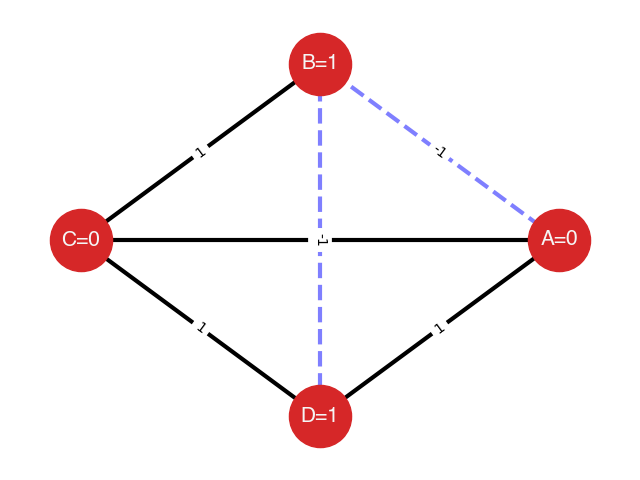
\includegraphics[width=0.7\linewidth]{Figures/entree-[0, 1, 0, 1].png}
        \caption{Configuration d'entrée \texttt{[0, 1, 0, 1]}}
        \label{fig:entree}
    \end{figure}
\end{enumerate}

\section{Annexes}
\subsection{\texttt{Code développé en Python}}
\begin{minted}{python}
from numpy import array, zeros
import numpy as np
import matplotlib.pyplot as plt
import random
from random import randrange
import networkx as nx
import math

...Plus de code ici
\end{minted}
\fi

\section{CM 1}

\subsection{Notations}
\begin{itemize}
	\item Observations are described by $p$ \hl{features} $\bm{X}=(X_{1},...,X_{p})\in\mathit{E}$ $ (E=\mathbb{R}^{p},...)$
	\item $\bm{X}_{i}=(X_{i1},...,X_{ip})$ is the features for observation $i$ $(1 \leq i \leq n)$
	\item $\mathit{Z}_i\in\{1,...,\mathit{K}\}$ is the \hl{group} of observation $i$
\end{itemize}

\subsection{The Mixture Model}
\textbf{Idea:} each group is described by its \textit{own} probability distribution.
\[
\bm{X} \mid \mathit{Z} = k \sim f(\mathbf{x},\theta_{k})=f_k(\mathbf{x})
\]

\textbf{How to read it:}
\begin{itemize}
\item $\bm{X}$ = feature vector describing one observation.
\item $Z=k$ = the observation belongs to group/cluster $k$.
\item $\bm{X}\mid Z=k$ = the features \emph{given that} the observation belongs to group $k$.
\item $\sim$ = ``is distributed according to''.
\item $f_k(\mathbf{x})$ = the probability distribution (density) for group $k$.
\item $\theta_k$ = parameters describing the distribution for group $k$.
\end{itemize}

\textbf{In words:}
\[
\boxed{\text{If an observation belongs to group }k,
\text{ its features follow the distribution }f_k
\text{ with parameters }\theta_k.}
\]

\textbf{Key idea:} Each group has its \emph{own} probability distribution:
\[
f_1(\mathbf{x}),;f_2(\mathbf{x}),;\ldots,;f_K(\mathbf{x}).
\]

\textbf{Important for clustering:} We observe $\bm{X}_i$, but $Z_i$ is typically
\emph{unknown}. We therefore use the observed features to infer which group
generated each observation.

\subsection{Mixing Proportions and Latent Group Membership}

The probability that an observation belongs to group $k$ is called the
\hl{mixing proportion}:

$$
p_k=P(Z=k),
\qquad k=1,\ldots,K.
$$

The mixing proportions satisfy

$$
p_k\geq 0
\qquad\text{and}\qquad
\sum_{k=1}^K p_k=1.
$$

Thus, $p_k$ represents the proportion (or prior probability) of observations
belonging to group $k$.

\medskip

\textbf{One-hot representation of the group membership:}

The group variable $Z$ can be represented by a vector
$\tilde{Z}=(\tilde{Z}_1,\ldots,\tilde{Z}_K)$ such that

$$
Z=k
\quad\Longleftrightarrow\quad
\tilde{Z}=(0,\ldots,0,1,0,\ldots,0),
$$

where the $1$ is in the $k$-th position. Therefore,

$$
\tilde{Z}_k=
\begin{cases}
1 & \text{if } Z=k,\\
0 & \text{otherwise.}
\end{cases}
$$

The membership vector follows a multinomial distribution with one trial:

$$
\tilde{Z}\sim\mathcal{M}(1,p_1,\ldots,p_K),
$$

and

$$
p_k=P(Z=k)=P(\tilde{Z}_k=1).
$$

\textbf{Key idea:} First, a group is selected according to the mixing
proportions $p_1,\ldots,p_K$. Then, the observation is generated from the
corresponding group distribution.

\subsection{Marginal Distribution of X: Mixture Density}
$\bm{X}$
Conditionally on belonging to group $k$,

$$
\bm{X}\mid Z=k\sim f_k(\mathbf{x}).
$$

Since $Z$ is generally unobserved, the marginal distribution of $\bm{X}$ is
obtained by combining all group distributions:

$$
\boxed{
f(\mathbf{x})
=
\sum_{k=1}^K p_k f_k(\mathbf{x})
}
$$

This is called the \hl{mixture density}.

$$
\boxed{
\text{Mixture density}
=
\sum
\text{mixing proportion}
\times
\text{group density}
}
$$

\subsection{Posterior Probability of Group Membership}

For an observed feature vector $\bm{X}=\mathbf{x}$, we want to compute the
probability that it belongs to group $k$:

$$
P(Z=k\mid \bm{X}=\mathbf{x}).
$$

Using Bayes' theorem:

$$
\boxed{
P(Z=k\mid \bm{X}=\mathbf{x})
=
\frac{p_kf_k(\mathbf{x})}
{\displaystyle\sum_{\ell=1}^K p_\ell f_\ell(\mathbf{x})}
=
\frac{p_kf_k(\mathbf{x})}{f(\mathbf{x})}
}
$$

\textbf{Interpretation:}
\begin{itemize}
\item $p_k$: how common group $k$ is (\textit{prior probability});
\item $f_k(\mathbf{x})$: how well group $k$ explains the observation
$\mathbf{x}$;
\item $P(Z=k\mid\bm{X}=\mathbf{x})$: the probability that the observation
belongs to group $k$ \emph{after observing} $\mathbf{x}$ (\textit{posterior
probability}).
\end{itemize}

\textbf{Memory aid:}

$$
\boxed{
\text{Prior probability}
\times
\text{How well the group explains }\mathbf{x}
\;\longrightarrow\;
\text{Posterior probability}
}
$$

\subsection{Classification Rule}

A \hl{classification rule} assigns each observation $\mathbf{x}\in E$ to one
of the $K$ groups:

$$
r:E\rightarrow\{1,\ldots,K\}.
$$

The rule is equivalent to partitioning the feature space $E$ into $K$
regions:

$$
\Omega_k=\{\mathbf{x}\in E:r(\mathbf{x})=k\},
$$

so that

$$
E=\bigcup_{k=1}^K\Omega_k,
\qquad
\Omega_k\cap\Omega_l=\varnothing\quad(k\neq l).
$$

\textbf{Interpretation:} $\Omega_k$ is the region of feature space that the
classifier assigns to group $k$.

\subsection{Classification Errors}

If an observation truly belongs to group $G_k$, the probability of classifying
it as group $G_l$ ($l\neq k$) is

$$
\boxed{
P(r(\mathbf{X})=l\mid Z=k)
=
P(\mathbf{X}\in\Omega_l\mid Z=k)
=
\int_{\Omega_l}f_k(\mathbf{x})\,d\mathbf{x}
}
$$

The probability of misclassifying an observation from group $G_k$ is

$$
\boxed{
P(r(\mathbf{X})\neq k\mid Z=k)
=
\sum_{l\neq k}P(r(\mathbf{X})=l\mid Z=k)
}
$$

The \hl{global probability of misclassification} (global classification
error) is

$$
\boxed{
P(r(\mathbf{X})\neq Z)
=
\sum_{k=1}^K
p_kP(r(\mathbf{X})\neq k\mid Z=k)
}
$$

\subsection{Cost and Risk}

Let $C_{kl}$ be the cost of classifying an observation from true group
$G_l$ as group $G_k$. Usually,

$$
C_{kk}=0.
$$

The \hl{conditional risk} of assigning an observation $\mathbf{x}$ to group
$k$ is the expected cost:

$$
\boxed{
R(k\mid\mathbf{x})
=
\sum_{l=1}^K
C_{kl}P(Z=l\mid\mathbf{X}=\mathbf{x})
}
$$

The \hl{average risk} of a classification rule $r$ is

$$
\boxed{
R(r)=\mathbb{E}[C_{r(\mathbf{X}),Z}]
}
$$

\textbf{Interpretation:}

$$
\boxed{
\text{Risk}=\text{expected cost of classification errors}
}
$$

\subsection{Bayes Optimal Classification Rule}

The \hl{Bayes optimal rule} is the rule that minimizes the average risk:

$$
\boxed{
r^*=\arg\min_r R(r)
}
$$

Equivalently, for each observation $\mathbf{x}$, choose the group with the
smallest conditional risk:

$$
\boxed{
r^*(\mathbf{x})
=
\arg\min_k R(k\mid\mathbf{x})
}
$$

\subsection{Bayes Rule with Equal Costs}

If every incorrect classification has the same cost,

$$
C_{kl}=
\begin{cases}
0 & k=l,\\
1 & k\neq l,
\end{cases}
$$

then minimizing conditional risk is equivalent to maximizing the posterior
probability:

$$
\boxed{
r^*(\mathbf{x})
=
\arg\max_k P(Z=k\mid\mathbf{x})
}
$$

Using Bayes' theorem,

$$
P(Z=k\mid\mathbf{x})
=
\frac{p_kf_k(\mathbf{x})}
{\displaystyle\sum_{l=1}^Kp_lf_l(\mathbf{x})},
$$

so equivalently,

$$
\boxed{
r^*(\mathbf{x})
=
\arg\max_k p_kf_k(\mathbf{x})
}
$$

\subsection{Bayes Rule for Two Groups}

For $K=2$:

$$
r^*(\mathbf{x})=
\begin{cases}
1 & \text{if }p_1f_1(\mathbf{x})>p_2f_2(\mathbf{x}),\\
2 & \text{otherwise.}
\end{cases}
$$

The decision boundary is given by

$$
\boxed{
p_1f_1(\mathbf{x})=p_2f_2(\mathbf{x})
}
$$

\subsection{Gaussian Mixture Model (GMM)}

A \hl{Gaussian Mixture Model} assumes that each group has a multivariate
Gaussian distribution:

$$
\boxed{
\mathbf{X}\mid Z=k
\sim
\mathcal{N}(\boldsymbol{\mu}_k,\Sigma_k)
}
$$

Thus,

$$
f_k(\mathbf{x})
=
\mathcal{N}(\mathbf{x};
\boldsymbol{\mu}_k,\Sigma_k).
$$

The marginal mixture density is

$$
\boxed{
f(\mathbf{x})
=
\sum_{k=1}^K
p_k\mathcal{N}(\mathbf{x};
\boldsymbol{\mu}_k,\Sigma_k)
}
$$

Each group is characterized by

$$
\boxed{
p_k,\quad\boldsymbol{\mu}_k,\quad\Sigma_k
}
$$

where $p_k$ is the mixing proportion, $\boldsymbol{\mu}_k$ the mean, and
$\Sigma_k$ the covariance matrix.

\subsection{Maximum Likelihood Estimation (MLE)}

Given observations $\mathbf{x}_1,\ldots,\mathbf{x}_n$, MLE chooses the
parameters that make the observed data most likely:

$$
\boxed{
\hat{\theta}
=
\arg\max_\theta L(\theta)
}
$$

where the likelihood is

$$
L(\theta)
=
\prod_{i=1}^n f(\mathbf{x}_i;\theta).
$$

\subsection{Log-Likelihood}

Because products are difficult to optimize, we use the logarithm:

$$
\boxed{
\ell(\theta)
=
\log L(\theta)
=
\sum_{i=1}^n
\log f(\mathbf{x}_i;\theta)
}
$$

Since $\log$ is increasing,

$$
\arg\max_\theta L(\theta)
=
\arg\max_\theta\ell(\theta).
$$

\subsection{Empirical Estimates}

If the group memberships are known, let

$$
\tilde Z_{ik}=
\begin{cases}
1 & \text{if observation }i\text{ belongs to group }k,\\
0 & \text{otherwise.}
\end{cases}
$$

Then

$$
n_k=\sum_{i=1}^n\tilde Z_{ik}
$$

is the number of observations in group $k$.

The usual empirical estimates are

$$
\boxed{
\hat p_k=\frac{n_k}{n}
}
$$

$$
\boxed{
\hat{\boldsymbol{\mu}}_k
=
\frac{1}{n_k}
\sum_{i=1}^n
\tilde Z_{ik}\mathbf{x}_i
}
$$

and

$$
\boxed{
\hat\Sigma_k
=
\frac{1}{n_k}
\sum_{i=1}^n
\tilde Z_{ik}
(\mathbf{x}_i-\hat{\boldsymbol{\mu}}_k)
(\mathbf{x}_i-\hat{\boldsymbol{\mu}}_k)^T
}
$$

\textbf{Important:} These estimates assume that the group memberships
$\tilde Z_{ik}$ are known. In unsupervised GMM clustering, the memberships
are unknown and must be estimated, which leads to methods such as
Expectation-Maximization (EM).

\subsection{Key Connections}

$$
\boxed{
\text{GMM}
\rightarrow
p_k,f_k(\mathbf{x})
\rightarrow
P(Z=k\mid\mathbf{x})
\rightarrow
\text{classification}
\rightarrow
\text{risk}
\rightarrow
\text{Bayes optimal rule}
}
$$

$$
\boxed{
\text{MLE}
\rightarrow
\text{estimate }p_k,\boldsymbol{\mu}_k,\Sigma_k
\rightarrow
\text{fit the GMM}
}
$$

\textbf{Memory aids:}
\begin{itemize}
\item \textbf{Classification rule:} ``Which group do I assign $\mathbf{x}$ to?''
    \item \textbf{Risk:} ``How costly is my decision?''
\item \textbf{Bayes rule:} ``Choose the decision with the smallest expected cost.''
    \item \textbf{Equal costs:} ``Choose the group with the highest posterior probability.''
\item \textbf{GMM:} ``Each group is a Gaussian with its own $p_k,\mu_k,\Sigma_k$.''
    \item \textbf{MLE:} ``Choose parameters that make the observed data most likely.''
\end{itemize}

\subsection{Proofs of Estimators}

$p$: number of features = 1 -> 1-dimensional GMM

\[
\tilde{Z} \sim \mathcal{M}(1,p_1,...,p_k)
\]
\[
X \mid Z = k \sim \mathcal{N}(\mu_p, \sigma_{pk}^2)
\]
\[
\theta = p_k, \mu_k, \sigma_k^2
\]
\[
k=1,...,K
\]
\[
f_k(.) = \frac{1}{\sqrt{2\pi\sigma_k^2}}exp(-\frac{1}{2}(\frac{x-\mu_k}{\sigma_k})^2)
\]
\[
\underline{X} = (X_1,...,X_n)
\]
\[
\underline{Z} = (Z_1,...,Z_n)
\]
\[
\ln\mathbf{L}(\underline{X}, Z, \theta) = \sum_{i=1}^{n} \sum_{k=1}^{K} \tilde{Z}_{ik}(\ln p_k -\frac{1}{2}(\ln \sigma_k^2) -\ln\sqrt{2\pi} -\frac{1}{2}(\frac{(x-\mu_k)^2}{\sigma_k^2})
\]
\[
\sum_{k=1}^K p_k = 1 \implies \sum_{k=1}^K p_k - 1 = 0
\]
\[
\sum_{k=1}^K p_k - 1 = \psi(x)
\]
Pour trouver l'extraminum de $\phi(x)$, $x \in \mathbb{R}^n$, sous la contrainte $\psi(x) = 0$, on optimise :
\[
F(x, \lambda) = \phi(x)+\lambda \psi(x)
\]
en $(x, \lambda)$, ce qui nous donne l'optimum $(x^*, \lambda^*)$
\[
F(p_k, \lambda) = \sum_{i=1}^{n} \sum_{k=1}^{K} \tilde{Z}_{ik}(\ln p_k + ...) + \lambda(1 - \sum_{k=1}^K p_k)
\]

\begin{enumerate}
	\item $\frac{\partial F(p_k, \lambda)}{\partial p_k} = 0$
	\item $\frac{\partial F(p_k, \lambda)}{\partial \lambda} = 0$
\end{enumerate}





\section{Univariate vs. Multivariate Gaussian Distributions}

This section compares the mathematical definitions and structural components of the 1D (univariate) and multi-dimensional (multivariate) Gaussian distributions.

\subsection{Probability Density Functions (PDFs)}

\subsubsection{Univariate Gaussian Distribution}
For a single continuous random variable $x$, the probability density function is defined as:
\begin{equation}
f(x) = \frac{1}{\sqrt{2\pi\sigma^2}} \exp\left( -\frac{(x - \mu)^2}{2\sigma^2} \right)
\end{equation}
Where:
\begin{itemize}
    \item $\mu$ is the scalar mean (location of the peak).
    \item $\sigma^2$ is the scalar variance (spread of the distribution).
\end{itemize}

\subsubsection{Multivariate Gaussian Distribution}
For a $D$-dimensional vector of random variables $\mathbf{x} = [x_1, x_2, \dots, x_D]^T$, the probability density function generalizes to:
\begin{equation}
f(\mathbf{x}) = \frac{1}{\sqrt{(2\pi)^D |\boldsymbol{\Sigma}|}} \exp\left( -\frac{1}{2} (\mathbf{x} - \boldsymbol{\mu})^T \boldsymbol{\Sigma}^{-1} (\mathbf{x} - \boldsymbol{\mu}) \right)
\end{equation}
Where:
\begin{itemize}
    \item $\boldsymbol{\mu} \in \mathbb{R}^D$ is the mean vector.
    \item $\boldsymbol{\Sigma} \in \mathbb{R}^{D \times D}$ is the symmetric, positive-definite covariance matrix.
    \item $|\boldsymbol{\Sigma}|$ denotes the determinant of the covariance matrix.
    \item $\boldsymbol{\Sigma}^{-1}$ is the inverse of the covariance matrix.
\end{itemize}

\subsection{Mathematical Component Mapping}

The table below illustrates how the components of the univariate formula scale up to handle multiple dimensions.

\begin{table}[h!]
\centering
\small
\caption{Structural Translation from 1D to D-Dimensions}
\label{tab:gaussian_comparison}
\begin{tabularx}{\textwidth}{p{2.6cm} p{2.4cm} p{3.2cm} X}
\hline
\textbf{Component} & \textbf{Univariate (1D)} & \textbf{Multivariate ($D$-D)} & \textbf{Structural Role} \\ \hline
Input Variable & Scalar: $x$ & Vector: $\mathbf{x} \in \mathbb{R}^D$ & Tracks multiple dimensions simultaneously. \\ \hline
Center / Mean & Scalar: $\mu$ & Vector: $\boldsymbol{\mu} \in \mathbb{R}^D$ & Contains individual coordinates for the center. \\ \hline
Spread / Scale & Variance: $\sigma^2$ & Matrix: $\boldsymbol{\Sigma} \in \mathbb{R}^{D \times D}$ & Determinant $|\boldsymbol{\Sigma}|$ scales the density volume. \\ \hline
Inverse Spread & Division: $\frac{1}{\sigma^2}$ & Matrix Inverse: $\boldsymbol{\Sigma}^{-1}$ & Matrix inversion replaces regular division. \\ \hline
Distance Metric & $(x - \mu)^2$ & $(\mathbf{x} - \boldsymbol{\mu})^T \boldsymbol{\Sigma}^{-1} (\mathbf{x} - \boldsymbol{\mu})$ & Computes squared Mahalanobis distance. \\ \hline
Normalization & $\sqrt{2\pi\sigma^2}$ & $\sqrt{(2\pi)^D |\boldsymbol{\Sigma}|}$ & Scales total density volume to integrate to 1. \\ \hline
\end{tabularx}
\end{table}

\subsection{Key Geometric Interpretation}
The exponent term in the multivariate PDF represents the \textit{Mahalanobis distance}. Unlike the standard Euclidean distance, it accounts for variances along each axis and covariances between dimensions. This turns the perfectly circular or spherical contours of independent variables into multi-dimensional hyperellipsoids when variables correlate.


\end{document}